\documentclass[final, xcolor=cmyk]{beamer}
\mode<presentation>

% STEP 1: Change the next line according to your language
\usepackage[english]{babel}
\usepackage{multicol}
\usepackage{fontspec}

% STEP 2: Make sure this character encoding matches the one you save this file as
% (this template is utf8 by default but your editor may change it, causing problems)
\usepackage[utf8x]{inputenc}
\usepackage{graphicx}
% You probably don't need to touch the following four lines
\usepackage[T1]{fontenc}
\usepackage{lmodern}
\usepackage{amsmath,amsthm, amssymb, latexsym}
\usepackage{calc}
\usepackage{exscale} % required to scale math fonts properly
\usepackage{eulervm} % Euler VM symbols
%\usepackage[cmbrightmath,scaleupmath]{tpslifonts}
%\usepackage{cmbright} % CM Bright math
\usepackage{ragged2e} 
\usepackage{svg}
\usepackage{subfigure}
\usepackage{booktabs}
\graphicspath{{images/}}
%\usepackage[orientation=portrait,size=a0,scale=1.3]{beamerposter}
\usepackage[orientation=portrait,size=custom,width=90,height=120,scale=1.2]{beamerposter}

\usepackage{tikz}
\newcommand*\circled[1]{\tikz[baseline=(char.base)]{
        \node[shape=circle,draw,inner sep=2pt] (char) {#1};}}


% STEP 3:
% Change colours by setting \usetheme[<id>, twocolumn]{LETI}.
\usetheme[color, twocolumn]{LETI}

%\setbeamertemplate{background}[grid]{}

% STEP 4: Set up the title and author info
\titlestart{$A^2$-Net: Molecular Structure Estimation from Cryo-EM Density Volumes} % first line of title
\titleend{} % second line of title
%\titlesize{\Huge} % Use this to change title size if necessary

\author{Kui Xu, Zhe Wang, Jianping Shi, Hongsheng Li, Qiangfeng Cliff Zhang}
\institute{School of Life Sciences, Tsinghua University}


% Stuff such as logos of contributing institutes can be put in the lower left corner using this
\leftcorner{}

\newcommand{\figfont}{\normalsize} % set fotsize for figures 

\begin{document}
\begin{poster}
%%%%%%%%%%%%%%%%%%%%%%%%%%%%%%%%%%%%%%%%%%%%%%%%%%%%%%%%%%%%%%%%%%%%%%%%%%%%%%
% First column %%%%%%%%%%%%%%%%%%%%%%%%%%%%%%%%%%%%%%%%%%%%%%%%%%%%%%%%%%%%%%%
\newcolumn
\section{Abstract}
\justifying
Constructing of molecular structural models from Cryo- Electron Microscopy (Cryo-EM) density volumes is the critical last step of structure determination by Cryo-EM technologies. 
Methods have evolved from manual construction by structural biologists to perform 6D translation-rotation searching, which is extremely compute-intensive. 
\begin{itemize} 
    \justifying
    \item In this paper, we propose a learning-based method and formulate this problem as a vision-inspired 3D detection and pose estimation task. 
    \item We develop a deep learning framework for amino acid determination in a 3D Cryo-EM density volume. 
    \item We also design a sequence-guided Monte Carlo Tree Search (MCTS) to thread over the candidate amino acids to form the molecular structure. This framework achieves 91\% coverage on our newly proposed dataset and takes only a few minutes for a typical structure with a thousand amino acids. 
\end{itemize}
Our method is hundreds of times faster and several times more accurate than existing automated solutions without any human intervention.


\section{The architecture of $A^2$-Net}
\begin{figure}
    \subfigure[The architecture of A2-Net.]{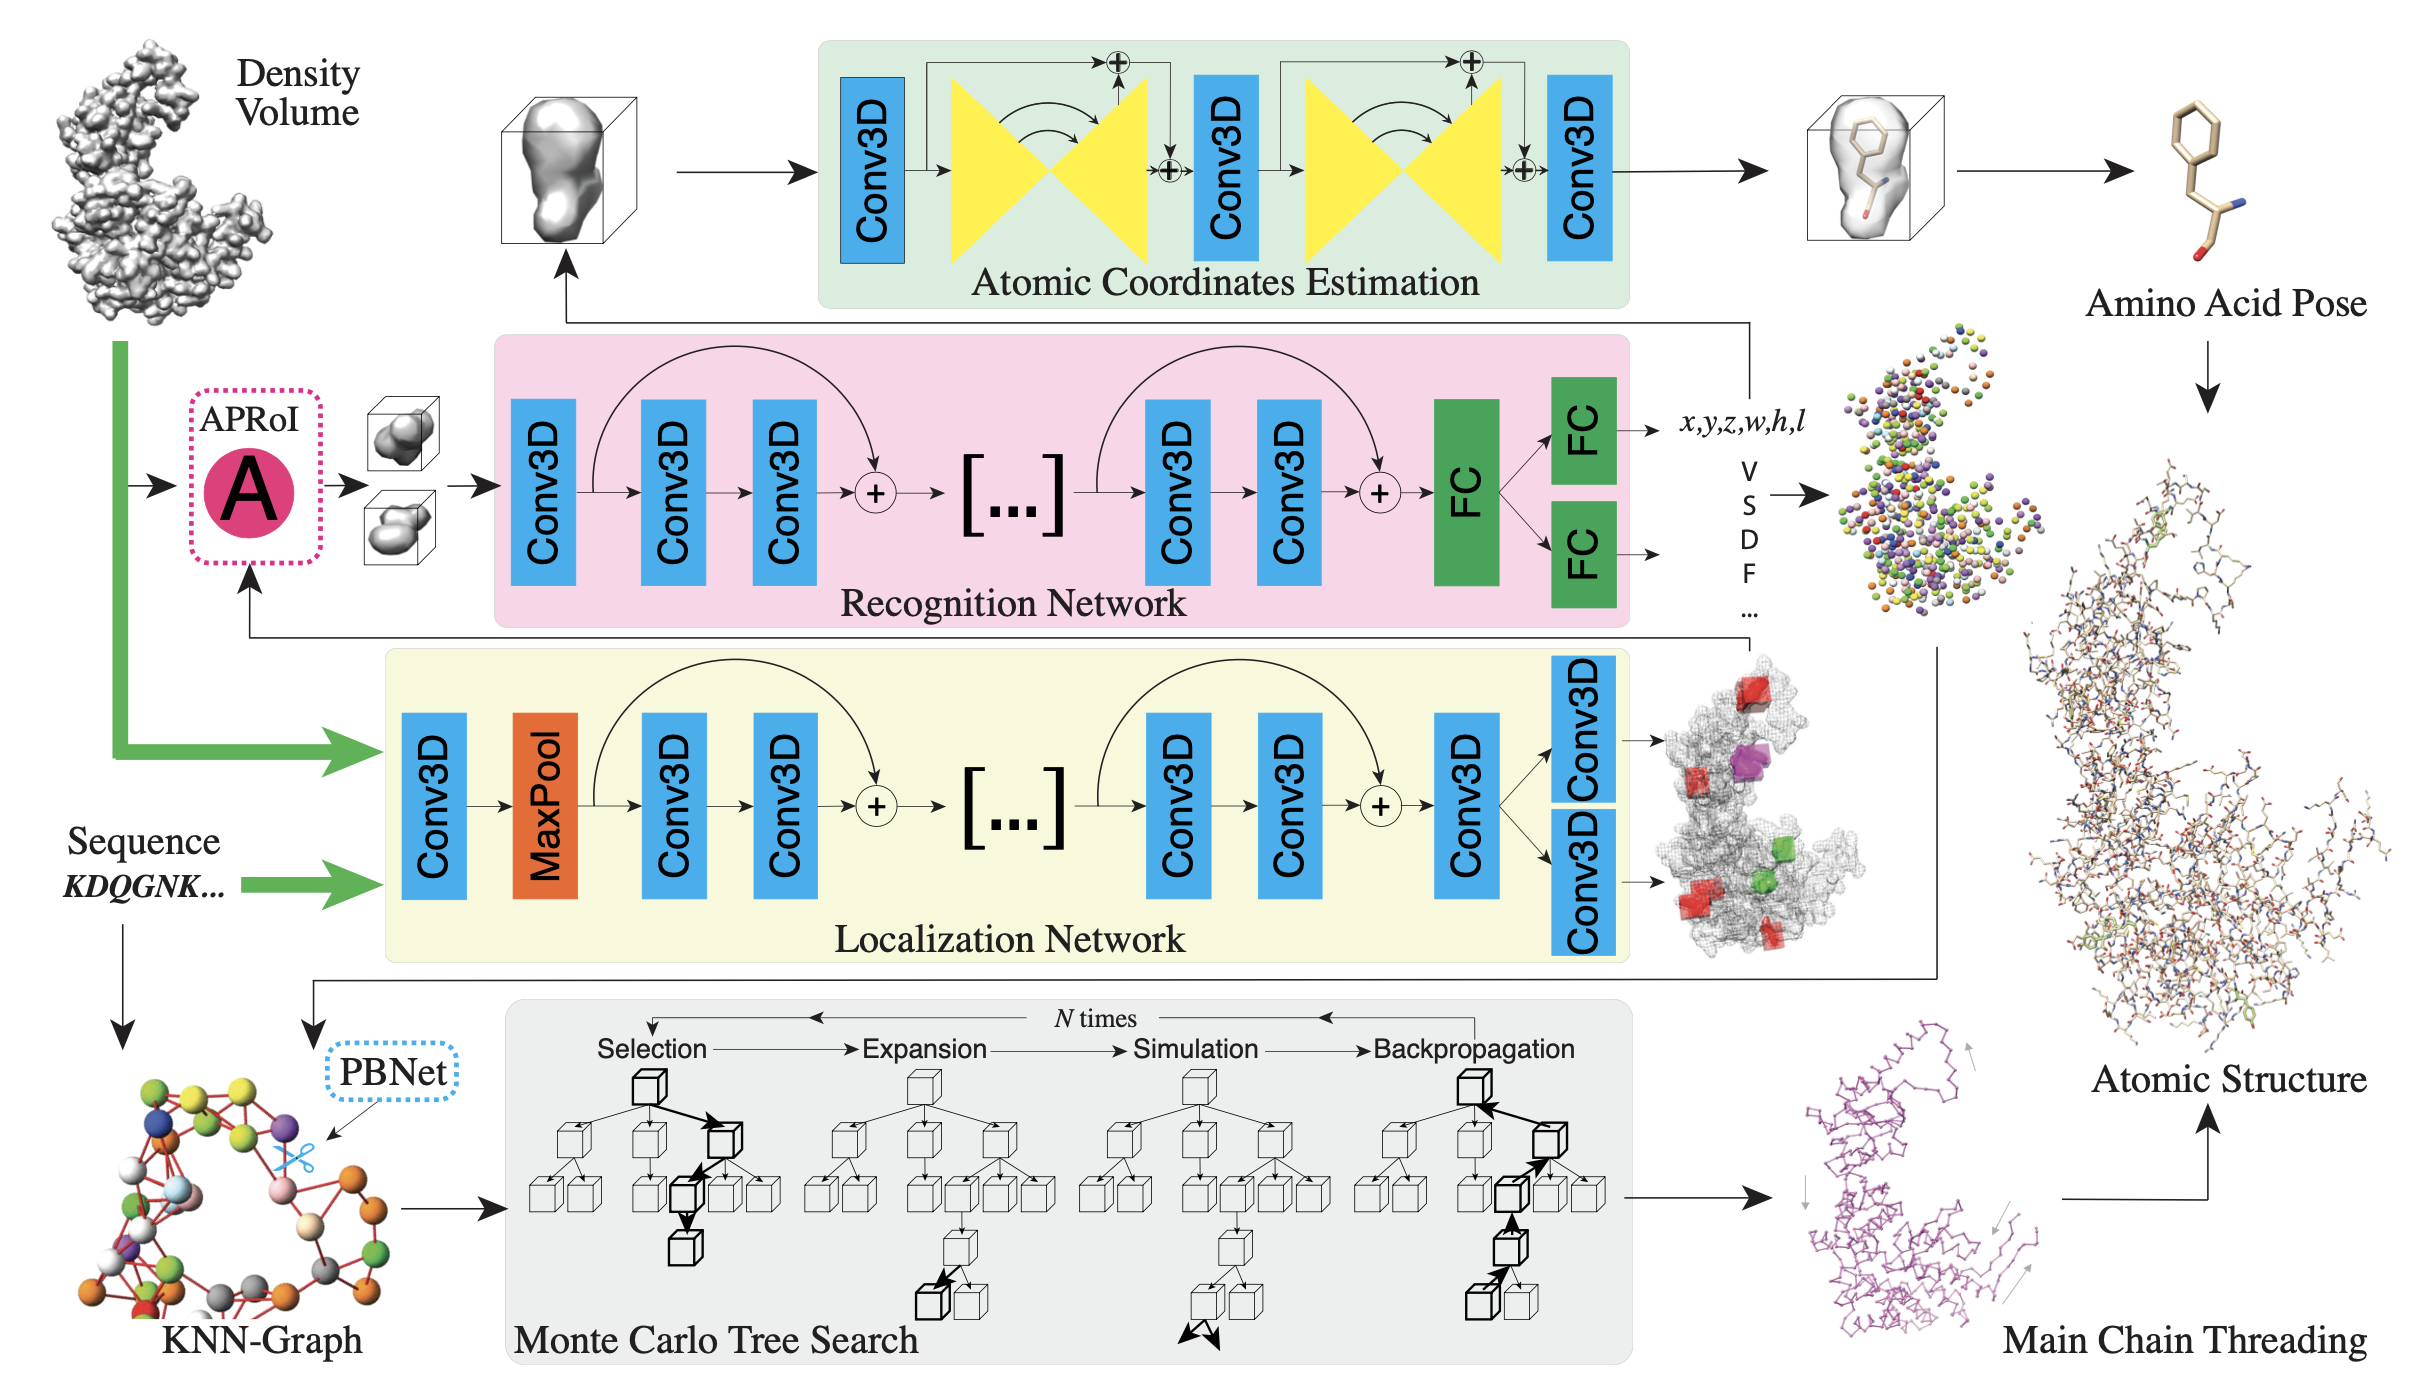
\includegraphics[width=0.9\columnwidth]{arch.png}}
\end{figure}
Given the density volume and the amino acid sequential orders, the localization network (locNet) and recognition network (recNet) locate and classify 20 types of amino acids in it. 
The atomic coordinates estimation network regresses the atomic coordinates. With the proposed amino acid, a MCTS algorithm is used for main chain threading.

\vspace*{1ex}
\subsection{3D Amino Acid Detection} \justifying
$A^2$- Net first obtains 3D feature volumes and generates 3D box proposals with the region proposal network (RPN)

\vspace*{1ex}
\subsection{3D Amino Acid Pose Estimation} \justifying
For an amino acid with $N$ atoms, poseNet produces $H$ estimated heatmaps with $N$ channels. The Mean Squared Error loss is adopted:
\begin{equation}
    L_{p o s e}=\sum_{h}^{H} \sum_{n}^{N}\left\|y_{h}^{*}(n)-y_{h}(n)\right\|_{2}^{2}
    \end{equation}
    where $y_{h}^{*}$ denotes the predicted heatmap by the $h$-th stack,
$n$ denotes the $n$-th atom, and $y_h$ is the ground-truth heatmap with the $N \times 8$ locations labeled.

\vspace*{1ex}
\subsection{Monte Carlo Tree Search for Threading} \justifying
A single iteration of the MCTS building process consists of four steps: 
\begin{itemize}
    \item selection: a node to be expanded is selected;
    \item expansion: the node is expanded by simulating the associated action;
    \item simulation: the tracing is simulated following a random path until the terminal amino acid is reached;
    \item back propagation: the result propagates back through the tree
\end{itemize}

\newcolumn
% Table generated by Excel2LaTeX from sheet 'Sheet1'

  
\section{Results} 
\subsection{Amino Acid Detection}
\begin{figure}[!htbp]
    \subfigure[The results of detection and threading comparing with other 3D object detection methods.]{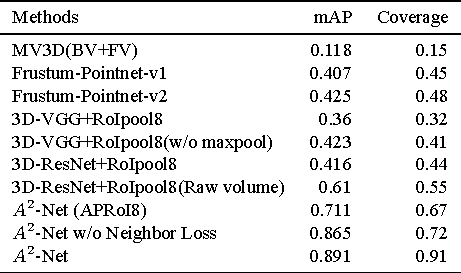
\includegraphics[scale=2.5]{detection_nowhite.pdf}}
    \subfigure[An example of amino acid detection result by $A^2$-Net.]{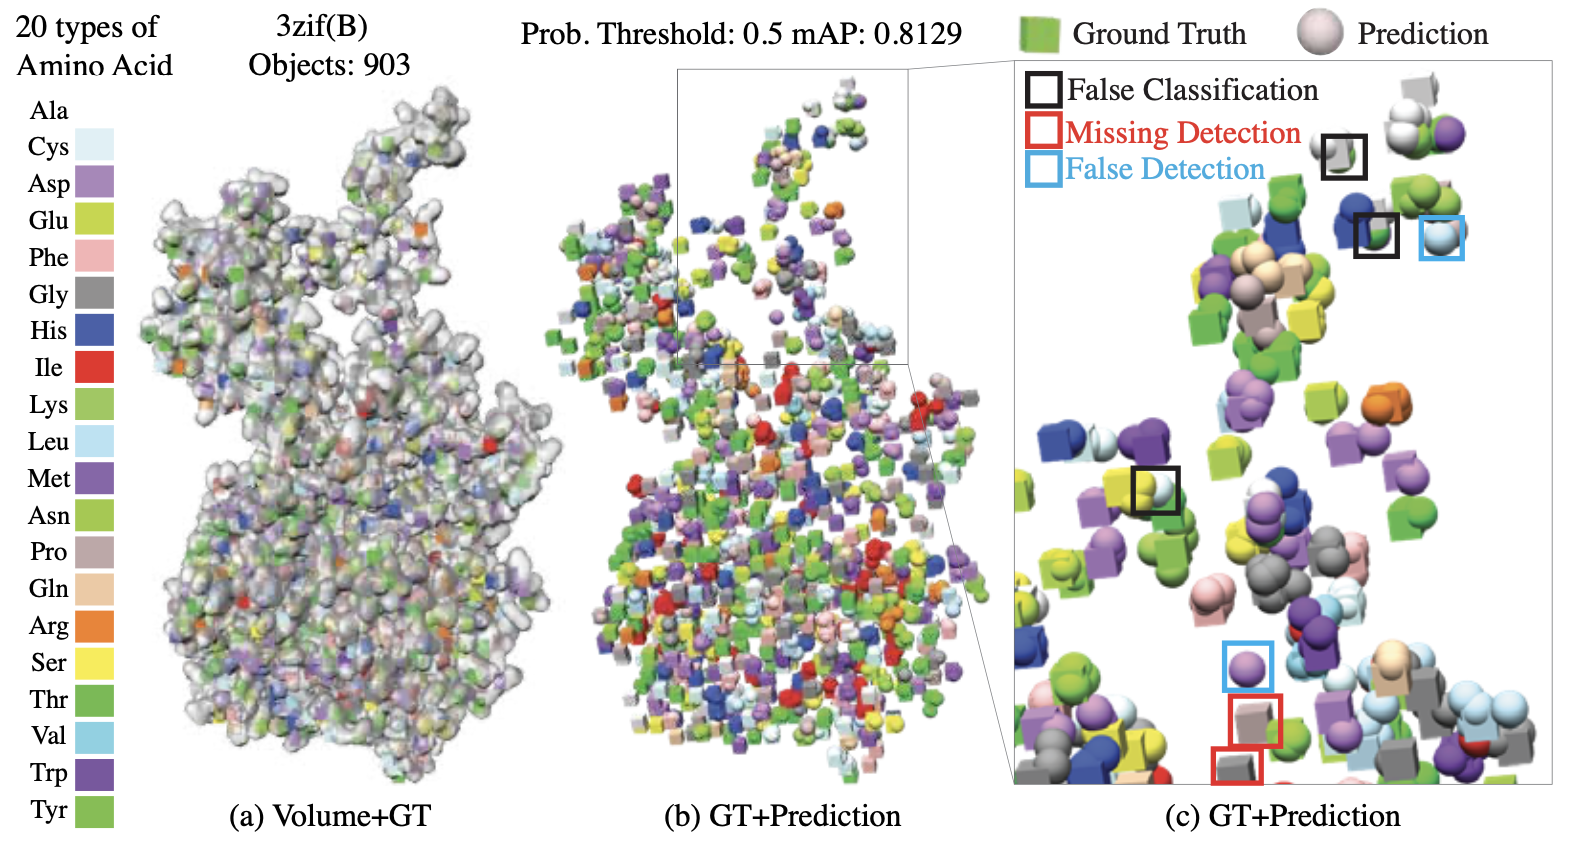
\includegraphics[width=0.45\columnwidth]{aadetection.png}}
    

\end{figure}
\begin{itemize}
    \item The category-specific information may be discarded in the feature map of the locNet model.
    \item Although the gain of mAP from neighbor loss was only marginal, the sequence coverage percentage of the threading result improved substantially.
    \item Our method outperformed them by a large margin during comparison with other 3D Detection Methods.
\end{itemize}
\subsection{Main Chain Threading}
\begin{figure}
    \subfigure[The results of threading by DFS-based methods and the proposed MCTS+PBNet.]{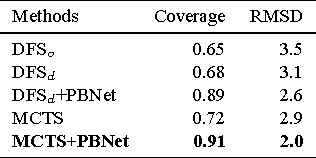
\includegraphics[scale=2.5]{thread1_nowhite.pdf}}
    \subfigure[Threading accuracy and efficiency compared with Rosetta-denovo. R1 and R2 denotes round 1 and 2.]{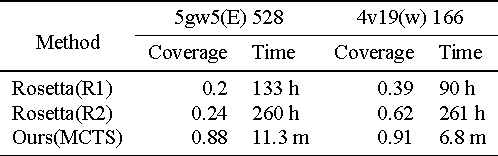
\includegraphics[scale=2.5]{thread2_nowhite.pdf}}
    \quad
    \subfigure[An example of threading results by MCTS+PBNet.]{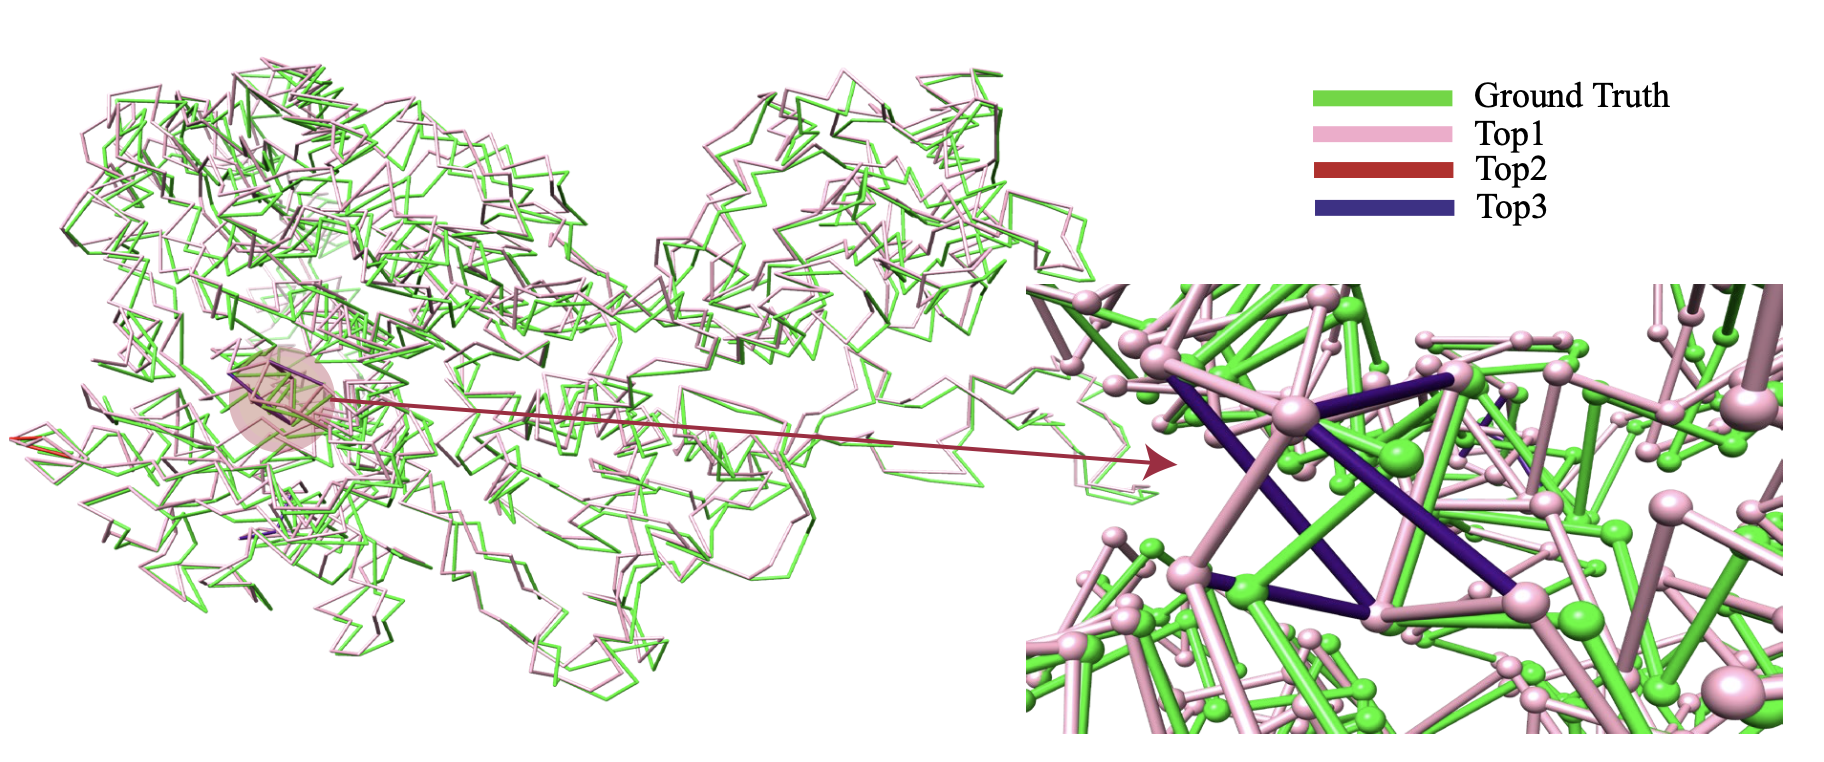
\includegraphics[width=0.9\columnwidth]{thread.png}}

    %\caption{Threading results by MCTS+PBNet}
\end{figure}
\begin{itemize}
    \item Both threading algorithms DFS and MCTS are largely improved with PBNet. 
    \item Rosetta-denovo is very time- consuming. 
\end{itemize}


\subsection{Generic Features for 3D Detection}
\begin{figure}
    \subfigure[The AP of different methods for 3D car detection on KITTI dataset w/ or w/o $A^2$ dataset]{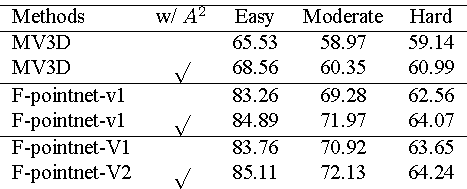
\includegraphics[scale=2.5]{AP_nowhite.pdf}}
\end{figure}
\section{Conclusion}
In this work, we reformulate the challenging molecular structure determination problem and propose a learning-based framework. 
\begin{itemize}
    \item The newly designed $A^2$-Net predicts accurate amino acid proposals with our APRoI layer and the neighbor loss training strategy. 
    \item With the predictions and the sequence, we propose a MCTS algorithm for efficient threading. 
    \item Using the peptide bond recognition network, tree branches between candidate pairs of proposals without a real peptide bond can be easily removed, which simultaneously improves the searching efficiency and the sequence coverage. 
    \item Our novel method is hundreds of times faster and more accurate than the previous method, and will play a vital role in molecular structure determination.
\end{itemize}
% \begin{table}[htbp]
%     \centering
%     \caption{Add caption}
%       \begin{tabular}{lrr}
%       Methods  & mAP & Coverage  \\
%       MV3D(BV+FV)  & 0.118 & 0.15 \\
%       Frustum-Pointnet-v1  & 0.407 & 0.45 \\
%       Frustum-Pointnet-v2  & 0.425 & 0.48 \\
%       3D-VGG+RoIpool8  & 0.36  & 0.32 \\
%       3D-VGG+RoIpool8(w/o maxpool)  & 0.423 & 0.41 \\
%       3D-ResNet+RoIpool8  & 0.416 & 0.44 \\
%       3D-ResNet+RoIpool8(Raw volume)  & 0.61  & 0.55 \\
%       A2-Net (APRoI8)  & 0.711 & 0.67 \\
%       A2-Net w/o Neighbor Loss  & 0.865 & 0.72 \\
%       A2 -Net  & 0.891 & 0.91 \\
%       \end{tabular}%
%     \label{tab:addlabel}%
%   \end{table}%

\end{poster}

\end{document}
% %%%%%%%%%%%%%%%%%%%%%%%%%%%%%%%%%%%%%%%%%%%%%%%%%%%%%%%%%%%%%%%%%%%%%%%%%%%%%%
% % First column %%%%%%%%%%%%%%%%%%%%%%%%%%%%%%%%%%%%%%%%%%%%%%%%%%%%%%%%%%%%%%%
% \newcolumn

% \section{Motivation}
% \justifying

% %Electrolyte barriers is used in CV measurements of InAs because formation of reliable Schottky contact is difficult due to surface accumulation.
% %Although this technique is widely used for characterisation of grate range of semiconductors, the electrolyte-based capacitance-voltage plots of InAs is differ form many other materials and use of depletion approximation give higher concentration compering to hall measurements.


% \begin{itemize} 
%     \justifying
%     \item Schottky contact is usually used in capacitance-voltage characterisation, but formation of reliable Schottky contact to InAs is difficult due to charge  accumulation at the surface.
%     \item Electrolyte can be used to form Schottky-like barrier junction to InAs, however, electrolyte based C-V measurements in n-InAs give overestimated impurity concentration.
% \end{itemize}
% % change line spacing

% The purpose of present work is to explain the mismatch between CV and Hall results and to determine the optimal parameters of CV measurements for doping density extraction in n-InAs.

% \vspace*{-2ex}
% \section{Semiconductor-electrolyte interface} \justifying


% \centering{
% \figfont
% \includesvg[clean, width=0.7\columnwidth]{images/sem_el}
% \includesvg[clean, width=0.45\columnwidth]{images/sem_el_cap}
% \vspace{1em}
% \caption{The structure of semiconductor-electrolyte interface}  
% }

% \vspace{3ex}
% \begin{columns}
%     \figfont
%     \newcommand{\figwidth}{0.5555\columnwidth}
%     \begin{column}{\figwidth}
%         \centering{
%         \includesvg[clean, width=0.7\columnwidth]{images/IP_band_edge1}
%         \caption{Position of energy bands at the surface of various semiconductors}
%         }
%     \end{column}
%     \begin{column}{\columnwidth-\figwidth}
%         \includesvg[clean, width=0.7\columnwidth]{images/IP_band_edge2}
%         \centering{
%         \caption{Band diagrams of InAs and \\ GaAs at equilibrium}
%         }
%     \end{column}
% \end{columns}
% \vspace{-2ex}

% \section{Simulation} \justifying
% %Capacitance-voltage characteristics were calculated from potential distributions obtained by solving Poisson equation with modified Thomas-Fermi approximation (MTFA).   

% Poisson equation with modified Thomas-Fermi approximation (MTFA) was used to calculate CV characteristics.
% \vspace*{-1ex}

% \subsection{Poisson equation}
% \vspace*{-1ex}
%     $$
%         \frac{d^2\varphi}{dz^2} =
%          -\frac{q}{\varepsilon\varepsilon_0}\left[N_D^+ - N_A^- - n(z) + \
%           p(z)\right] 
%     $$
    
%     with electron concentration:
%     $$
%         n(z) = \int_{0}^{\infty}\rho_c(z,E) f_{FD}(E) f_{MTFA}(z,E)dE
%     $$ 
    
%     and  DOS for non-parabolic conduction band:  
%     $$
%         \rho \left(z,E\right) = \frac{1}{2\pi^2} \left(\frac{2m_{e}}{\hbar^2}\right)^{3/2} \!\!\! \sqrt{E} \cdot \sqrt{1+\alpha E} \cdot \left(1+ 2\alpha E \right)
%     $$  
    
% %    $$
% %   \text{where}\ \alpha = \frac{1}{E_g}\left(1 - \frac{m_{\Gamma}}{m_0}\right)^{\!2}\ \ \text{--- nonparabolicity coefficient}
% %    $$

% \vspace{-1ex}       
% \subsection{Modified Thomas-Fermi approximation}
%     MTFA used to take into account boundary condition for wave function during accumulation.  
%     $$
%     f_{MTFA}(z, E)  = 1 - sinc\left( \frac{2z}{L} \left(\frac{E}{k_BT}\right)^{1/2} \left(1+\alpha E\right)^{1/2}\right)
%     $$
    
% %%%%%%%%%%%%%%%%%%%%%%%%%%%%%%%%%%%%%%%%%%%%%%%%%%%%%%%%%%%%%%%%%%%%%%%%%%%%%%
% % Second column %%%%%%%%%%%%%%%%%%%%%%%%%%%%%%%%%%%%%%%%%%%%%%%%%%%%%%%%%%%%%%
% \newcolumn

% \section{Results} \justifying
% \subsection{Energy band diagrams}
%         \centering{
%         \figfont
%         \includesvg[clean, width=\columnwidth]{images/IP_InAs_pot}
%         }
% \vspace*{-4ex}

% \subsection{Typical Mott-Schottky plot}
% \vspace{0.5ex}
% \newcommand{\figwidth}{0.545\columnwidth}
% \begin{columns}[c]
%     \begin{column}{0.95\columnwidth-\figwidth}
%         \begin{itemize}   \itemsep15pt    
%             \item  Linear fitting of $C^{-2}\,vs.\,V$ plot gives doping concentration.
%             \item Deep depletion can occur.
%             \item Deviation from linear behavior due to grows of parasitic conductance.
%         \end{itemize}

%         $$
%         \frac1{C^2}=\frac2{q\varepsilon\varepsilon_0 N_D} \
%                     \left( V- V_{FB} \right)
%         $$

%     \end{column}
    
%     \begin{column}{0.005\columnwidth}
%     \end{column}
    
%     \begin{column}{\figwidth}
%         \centering{
%         \figfont
%         \includesvg[clean, width=1.07\columnwidth]{images/IP_InAs_CV_fig3}
%         \vspace*{1ex}
%         \caption{\hskip50pt Mott-Schotky plot of n-GaAs} 
%        } 
%     \end{column}
% \end{columns}
% \vspace*{2ex}	

% \subsection{Mott-Schottky plots for n-InAs/electrolyte}
% \vspace{0.5ex}
% %\newcommand{\figwidth}{0.55\columnwidth}
% \begin{columns}[c]
%         \begin{column}{0.95\columnwidth-\figwidth}
%                 \begin{itemize}   \itemsep15pt       
%                     \item $N_D = 2\times10^{18}\ \mathsf{cm^{-3}}$ from Hall measurements. Same value used in simulation.
%                     \item Capacitance measurements frequency: $f_m=2\ \mathsf{kHz}$.
%                     \item Accumulation occurs at low positive slope.
%                     \item Depletion at linear region.
%                 \end{itemize}
%         \end{column}
        
%         \begin{column}{0.005\columnwidth}
%         \end{column}
        
%         \begin{column}{\figwidth}
%            \centering
%            \figfont
%            \includesvg[clean, width=1.07\columnwidth]{images/IP_InAs_CV_fig1}
%            \vspace*{1ex}
%            \caption{\hskip50pt Mott-Schotky plot of $n^+\!$-InAs}  
%         \end{column}
% \end{columns}
   
% \begin{columns}[c]
%         \begin{column}{0.95\columnwidth-\figwidth}
%             \begin{itemize}    \itemsep15pt          
%                 \item $N_D = 1\times10^{15}\ \mathsf{cm^{-3}}$
%                 \item $f_m=1\ \mathsf{MHz}$.
%                 \item Depletion voltage span is very small.
%                 \item Fermi level shifts toward the
%                 center of forbidden energy gap, and the inversion starts earlier.
%                \end{itemize}
%         \end{column}
        
%         \begin{column}{0.005\columnwidth}
%         \end{column}   
                   
%         \begin{column}{\figwidth}
%              \vspace{1ex} 
%              \centering
%              \figfont
%              \includesvg[clean, width=1.07\columnwidth]{images/IP_InAs_CV_fig2}
%              \vspace*{1ex}
%              \caption{\hskip50pt Mott-Schotky plot of epi-InAs}  
%         \end{column}
% \end{columns}	

% %With implementation of controlled dissolution one can perform electrochemical capacitance-voltage (ECV) profiling technique to plot doping 

% \section{Summary} \justifying
%     \begin{itemize} \itemsep12pt
%         \justifying
%         \item The behavior of semiconductor-electrolyte interface depends on relative position of  band edges to electrochemical potential in electrolyte. This cause formation of accumulation layer in low doped InAs at equilibrium.
%         \item     In heavily doped n-InAs ($\mathsf{N_D > 10^{18}\ cm^{-3}}$)  the depletion approximation gives true doping density with 10  \% accuracy.
%         \item At the lower doping levels a simulation of capacitance-voltage characteristics should be used         to estimate doping density.
%     \end{itemize}


% \end{poster}
% \end{document}